\documentclass{article}
\usepackage[utf8]{inputenc}
\usepackage[default]{raleway}
\usepackage[table]{xcolor}
\usepackage{booktabs} 
\usepackage{ragged2e}
\usepackage{pgf-pie, multirow, longtable, tikz, titlesec, comment, tabularx, makecell, float, listings, array, setspace, geometry, graphicx, xcolor, xparse, fancyvrb, relsize, fancyhdr, booktabs, hyperref, eurosym}
%\geometry{a4paper, left=2cm, right=2cm, top=2cm, bottom=2.5cm}

\renewcommand{\headrulewidth}{0pt}

% ----------------------------- Definizione tabella ---------------------------

\newcolumntype{C}[1]{>{\centering\arraybackslash}m{#1}}

% ------------------------------Metadati indice --------------------------------
\title{\textbf{\fontsize{30}{6}\selectfont Indice}}
\author{\fontsize{14}{6}\selectfont ByteOps}
\date{}

% -----------------------------Creazione footer --------------------------------
\pagestyle{fancy} 
\fancyhf{}
\renewcommand{\footrulewidth}{0.4pt} 
\lfoot{ 
    \parbox[c]{2cm}{\includegraphics[width=2cm]{../Images/logo.png}}
    \textcolor[RGB]{120, 120, 120}{$\cdot$ Piano di progetto}
}
\rfoot{\thepage}

% --------------------------Modifica formato hyperlinks ------------------------
\hypersetup{
    colorlinks=true,
    linkcolor=black,
    filecolor=black,      
    pdftitle={Piano di progetto},
    pdfpagemode=FullScreen,
}

\definecolor{responsabile}{RGB}{0,102,204}
\definecolor{amministratore}{RGB}{0,204,102}
\definecolor{analista}{RGB}{255,165,0}
\definecolor{progettista}{RGB}{255,0,0}
\definecolor{programmatore}{RGB}{128,0,128}
\definecolor{verificatore}{RGB}{255,192,203}

\definecolor{responsabile}{RGB}{0,102,204}
\definecolor{amministratore}{RGB}{0,204,102}
\definecolor{analista}{RGB}{255,165,0}
\definecolor{progettista}{RGB}{255,0,0}
\definecolor{programmatore}{RGB}{128,0,128}
\definecolor{verificatore}{RGB}{255,192,203}



\begin{document}
\pagestyle{fancy}
\begin{center}
    \includegraphics[width = 0.7\textwidth]{../Images/logo.png} \\
    \vspace{0.2cm}
    \textcolor[RGB]{60, 60, 60}{\textit{ByteOps.swe@gmail.com}} \\
    \vspace{1cm}
    \fontsize{16}{6}\selectfont Piano di progetto \\
    \vspace{0.5cm}
\end{center}

\section*{Informazioni documento}
\def\arraystretch{1.2}
\begin{tabular}{>{\raggedleft\arraybackslash}p{0.2\textwidth}|>{\raggedright\arraybackslash}p{0.6\textwidth}c}
    \hline
    \addlinespace
    \textbf{Redattori}      & A. Barutta             \\ & R. Smanio \\ & N. Preto \vspace{10pt} \\
    \textbf{Verificatori}   & E. Hysa                \\ & L. Skenderi \\ & D. Diotto \vspace{10pt} \\
    \textbf{Amministratore} & F. Pozza \vspace{10pt} \\
    \textbf{Destinatari}    & T. Vardanega           \\ & R. Cardin \vspace{10pt} \\
    \textbf{Partecipanti}   & A. Barutta             \\ & E. Hysa \\ & R. Smanio \\ & D. Diotto \\ & F. Pozza \\ & L. Skenderi \\ & N. Preto \vspace{10pt} \\
\end{tabular}
\pagebreak

% ------------------------- Changelog ----------------------------

\begin{tabular}{|C{1.5cm}|C{2cm}|C{2cm}|C{2cm}|C{5cm}|}
    \hline
    \textbf{Versione}                & \textbf{Data} & \textbf{Autore} & \textbf{Verificatore} & \textbf{Dettaglio}            \\
    \hline
    \label{Git_Action_Version} 0.0.4 & 10/11/2023 & A.Barutta & E.Hysa & Aggiunti sez. Pianificazione \\
    \hline
    0.0.3 & 07/11/2023 & E.Hysa & L.Skenderi & Aggiunti nuovi rischi attesi \\
    \hline
    0.0.2 & 05/11/2023 & E.Hysa & L.Skenderi & Aggiunta sez. rischi \\
    \hline 
    0.0.1 & 03/11/2023 & A.Barutta & E.Hysa & Prima impostazione documento\\
    \hline 
 
    
\end{tabular}

\pagebreak

% ------------------------- Generazione automatica indice ----------------------
\setstretch{1.5}
\maketitle
\thispagestyle{fancy}
\tableofcontents
\listoffigures % Indice delle figure
\setstretch{1.2}
\pagebreak

% ---------------------------- Inizio documento -------------------------------

\section{Introduzione}
\subsection{Scopo del documento}
Il presente documento ha lo scopo di identificare la metodologia di pianificazione e illustrare le modalità con cui il gruppo \textit{ByteOps} sta sviluppando il progetto assegnato, al fine di garantire efficacia ed efficienza nel processo di sviluppo.\\
I contenuti che vengono trattati sono:
\begin{itemize}
    \item Analisi dei rischi
    \item Assegnazione ruoli dei membri del gruppo
    \item Descrizione del modello adottato con relative motivazioni della scelta
\end{itemize}



\subsection{Scopo del capitolato}
Il Capitolato C6 affidato al gruppo, si prefigge come obiettivo la realizzazione di una piattaforma di monitoraggio di una \textit{"Smart City"} che consenta di avere sotto controllo lo stato di salute della città in modo tale da prendere decisioni veloci, efficaci ed analizzare poi gli effetti conseguenti.
A tale scopo il proponente richiede di simulare dei sensori posti in diverse aree per reperire informazioni relative alle condizioni della città. 
I dati trasmessi in tempo reale dai sensori devono poter essere memorizzati in modo tale da renderli disponibili per la visualizzazione tramite una dashboard, composta anche da widget e grafici, per una visione d'insieme delle condizioni della città in tempo reale. 
L'applicativo potrà consentire alle autorità locali di prendere decisioni informate e tempestive sulla gestione delle risorse e sull'implementazione di servizi e, inoltre, si potrebbe rivelare uno strumento essenziale per coinvolgere i cittadini nella gestione e nel miglioramento della città. 

\subsection{Glossario}
Per evitare possibili incomprensioni con la terminologia utilizzata, verrà utilizzato il seguente simbolo:
\begin{itemize}
    \item \textit{G}: indica un termine presente nel documento \textit{Glossario}.  
\end{itemize}
%Glossario da definire


\subsection{Riferimenti}
\subsubsection{Riferimenti informativi}
\begin{itemize}
    \item \href {https://www.math.unipd.it/~tullio/IS-1/2023/Progetto/C6.pdf} {Capitolato d'appalto C6 - InnovaCity}
    \item \href{https://www.math.unipd.it/~tullio/IS-1/2023/Dispense/T4.pdf} {Slide del corso di Ingegneria del Software - Gestione di progetto}
    \item \href{https://www.math.unipd.it/~tullio/IS-1/2023/Dispense/T2.pdf} {Slide del corso di Ingegneria del Software - Ciclo di vita del software}

\end{itemize}

\subsubsection{Riferimenti normativi}
\begin{itemize}
\item Norme di progetto
\item \href {https://www.math.unipd.it/~tullio/IS-1/2023/Dispense/PD2.pdf} {Regolamento del progetto didattico}
\end{itemize}


%--Il seguente documento è stato redatto con l'obiettivo di valutare e disaminare i potenziali rischi che il gruppo potrebbe affrontare nel corso delle attività di sviluppo del capitolato. In questo documento veranno esposti i vari rischi identificati, accompagnati da una relativa previsione di impatto che ciascuno di essi potrebbe avere e una possibile soluzione.
\section{Calendario di massima del progetto}
\subsection{Introduzione}
Il calendario di massima del progetto illustra le date previste per le revisioni del progetto
alla luce di quanto analizzato nelle sezioni:
\begin{itemize}
    \item Analisi dei rischi;
    \item Analisi dei requisiti;
    \item Pianificazione.
\end{itemize}
\subsection{Prima stesura 25/10/2023}
Il gruppo si pone come obiettivo temporale delle revisioni il seguente calendario:
\begin{table}[ht]
    \centering
    \begin{tabular}{|c|c|}
        \hline
        \textbf{Revisione} & \textbf{Data} \\
        \hline
        Requirements and Technology Baseline & 20/12/2023 \\
        Product Baseline  & 29/03/2024 \\
        Customer Acceptance & 30/05/2024 \\
        % Aggiungi altre revisioni e date secondo necessità
        \hline
    \end{tabular}
    \caption{Calendario delle Revisioni}
\end{table}
\section{Stima dei costi di realizzazione}
\subsection{Introduzione}
La stima dei costi di realizzazione è la stima del budget totale necessario per la realizzazione del progetto alla luce di quanto analizzato in :
\begin{itemize}
    \item Analisi dei rischi;
    \item Analisi dei requisiti;
    \item Preventivo costi e assunzioni impegni.
\end{itemize}

\subsection{Prima Stesura 25/10/2023}
\begin{center}
        
    \begin{tabular}{|C{3cm}|C{2cm}|C{2cm}|C{2cm}|C{2cm}|C{2cm}|}
        \hline

        \textbf{Ruoli} & \textbf{Costo orario} \linebreak \textit{(\euro\ / h)} & \textbf{Ore previste per ruolo} & \textbf{Ore previste per membro} & \textbf{Costo per ruolo} \linebreak \textit{(\euro\ )} \\
        \hline\hline
        
        Responsabile & 30 & 49 & 7 & 1470 \\
        \hline
        
        Amministratore & 20 & 49 & 7 & 980 \\
        \hline
        
        Analista & 25 & 63 & 9 & 1575 \\
        \hline 
        
        Progettista & 25 & 210 & 30 & 5250 \\ 
        \hline
        
        Programmatore & 15 & 105 & 15 & 1575 \\
        \hline
        
        Verificatore & 15 & 175 & 25 & 2625 \\
        \hline\hline
        
        \textbf{TOTALE} & - & 651 & 93 & 13475 \\
        \hline
    \end{tabular}
    \end{center}

    \begin{figure}[h]
        \centering
        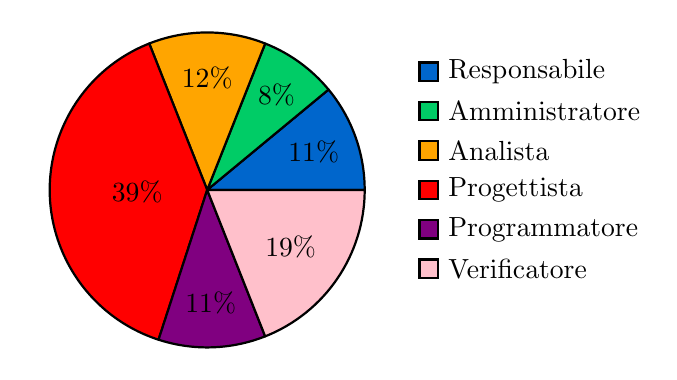
\begin{tikzpicture}
            \pie[
                text=legend,
                color={responsabile, amministratore, analista, progettista, programmatore, verificatore},
                radius=2, % Imposta il raggio per rendere il grafico circolare
                line width=0pt % Rimuovi i contorni
            ]{11/Responsabile, 8/Amministratore, 12/Analista, 39/Progettista, 11/Programmatore, 19/Verificatore}
        \end{tikzpicture}
        \caption{Distribuzione dei costi per ruolo}
    \end{figure}
    
    Il totale identificato di 13475\euro\ verrà considerato come limite di budget invalicabile,
    nel caso ci fosse il rischio di superamento del budget verranno negoziati al ribasso i requisiti
    di progetto.
\subsection{Seconda Stesura 16/12/2023}
Dopo una dettagliata rivalutazione dei requisiti e un'analisi con il committente, la stima dei costi è stata riesaminata. Ciò ha comportato la modifica delle ore dedicate alla progettazione e alla programmazione, portando così al nuovo costo di 12565\euro\ .
\begin{center}
        
    \begin{tabular}{|C{3cm}|C{2cm}|C{2cm}|C{2cm}|C{2cm}|C{2cm}|}
        \hline

        \textbf{Ruoli} & \textbf{Costo orario} \linebreak \textit{(\euro\ / h)} & \textbf{Ore previste per ruolo} & \textbf{Ore previste per membro} & \textbf{Costo per ruolo} \linebreak \textit{(\euro\ )} \\
        \hline\hline
        
        Responsabile & 30 & 49 & 7 & 1470 \\
        \hline
        
        Amministratore & 20 & 49 & 7 & 980 \\
        \hline
        
        Analista & 25 & 63 & 9 & 1575 \\
        \hline 
        
        Progettista & 25 & 140 & 20 & 3500 \\ 
        \hline
        
        Programmatore & 15 & 161 & 23 & 2415 \\
        \hline
        
        Verificatore & 15 & 175 & 25 & 2625 \\
        \hline\hline
        
        \textbf{TOTALE} & - & 651 & 93 & 12565 \\
        \hline
    \end{tabular}
    \end{center}

    \begin{figure}[h]
        \centering
        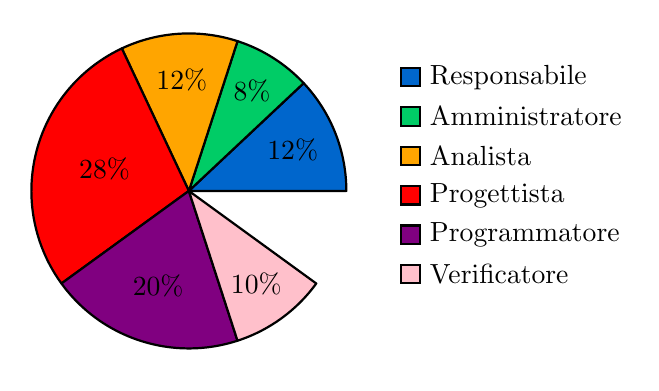
\begin{tikzpicture}
            \pie[
                text=legend,
                color={responsabile, amministratore, analista, progettista, programmatore, verificatore},
                radius=2, % Imposta il raggio per rendere il grafico circolare
                line width=0pt % Rimuovi i contorni
            ]{12/Responsabile, 8/Amministratore, 12/Analista, 28/Progettista, 20/Programmatore, 10/Verificatore}
        \end{tikzpicture}
        \caption{Distribuzione dei costi per ruolo aggiornamento 16/12/2023}
    \end{figure}


%--Il seguente documento è stato redatto con l'obiettivo di valutare e disaminare i potenziali rischi che il gruppo potrebbe affrontare nel corso delle attività di sviluppo del capitolato. In questo documento veranno esposti i vari rischi identificati, accompagnati da una relativa previsione di impatto che ciascuno di essi potrebbe avere e una possibile soluzione.
\section{Calendario di massima del progetto}
\subsection{Introduzione}
Il calendario di massima del progetto illustra le date previste per le revisioni del progetto
alla luce di quanto analizzato nelle sezioni:
\begin{itemize}
    \item Analisi dei rischi;
    \item Analisi dei requisiti;
    \item Pianificazione.
\end{itemize}
\subsection{Prima stesura 25/10/2023}
Il gruppo si pone come obiettivo temporale delle revisioni il seguente calendario:
\begin{table}[ht]
    \centering
    \begin{tabular}{|c|c|}
        \hline
        \textbf{Revisione}                   & \textbf{Data} \\
        \hline
        Requirements and Technology Baseline & 20/12/2023    \\
        Product Baseline                     & 29/03/2024    \\
        Customer Acceptance                  & 30/05/2024    \\
        % Aggiungi altre revisioni e date secondo necessità
        \hline
    \end{tabular}
    \caption{Calendario delle Revisioni}
\end{table}
\section{Stima dei costi di realizzazione}
\subsection{Introduzione}
La stima dei costi di realizzazione è la stima del budget totale necessario per la realizzazione del progetto alla luce di quanto analizzato in :
\begin{itemize}
    \item Analisi dei rischi;
    \item Analisi dei requisiti;
    \item Preventivo costi e assunzioni impegni.
\end{itemize}

\subsection{Prima Stesura 25/10/2023}
\begin{center}

    \begin{tabular}{|C{3cm}|C{2cm}|C{2cm}|C{2cm}|C{2cm}|C{2cm}|}
        \hline

        \textbf{Ruoli}  & \textbf{Costo orario} \linebreak \textit{(\euro\ / h)} & \textbf{Ore previste per ruolo} & \textbf{Ore previste per membro} & \textbf{Costo per ruolo} \linebreak \textit{(\euro\ )} \\
        \hline\hline

        Responsabile    & 30                                                     & 49                              & 7                                & 1470                                                   \\
        \hline

        Amministratore  & 20                                                     & 49                              & 7                                & 980                                                    \\
        \hline

        Analista        & 25                                                     & 63                              & 9                                & 1575                                                   \\
        \hline

        Progettista     & 25                                                     & 210                             & 30                               & 5250                                                   \\
        \hline

        Programmatore   & 15                                                     & 105                             & 15                               & 1575                                                   \\
        \hline

        Verificatore    & 15                                                     & 175                             & 25                               & 2625                                                   \\
        \hline\hline

        \textbf{TOTALE} & -                                                      & 651                             & 93                               & 13475                                                  \\
        \hline
    \end{tabular}
\end{center}

\begin{figure}[h]
    \centering
    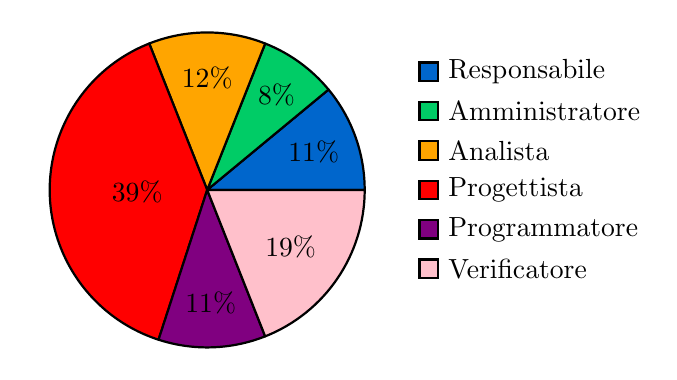
\begin{tikzpicture}
        \pie[
            text=legend,
            color={responsabile, amministratore, analista, progettista, programmatore, verificatore},
            radius=2, % Imposta il raggio per rendere il grafico circolare
            line width=0pt % Rimuovi i contorni
        ]{11/Responsabile, 8/Amministratore, 12/Analista, 39/Progettista, 11/Programmatore, 19/Verificatore}
    \end{tikzpicture}
    \caption{Distribuzione dei costi per ruolo}
\end{figure}

Il totale identificato di 13475\euro\ verrà considerato come limite di budget invalicabile,
nel caso ci fosse il rischio di superamento del budget verranno negoziati al ribasso i requisiti
di progetto.
\subsection{Seconda Stesura 16/11/2023}
Dopo una dettagliata rivalutazione dei requisiti e un'analisi con il committente, la stima dei costi è stata riesaminata. Ciò ha comportato la modifica delle ore dedicate alla progettazione e alla programmazione, portando così al nuovo costo di 12565\euro\ .
\begin{center}

    \begin{tabular}{|C{3cm}|C{2cm}|C{2cm}|C{2cm}|C{2cm}|C{2cm}|}
        \hline

        \textbf{Ruoli}  & \textbf{Costo orario} \linebreak \textit{(\euro\ / h)} & \textbf{Ore previste per ruolo} & \textbf{Ore previste per membro} & \textbf{Costo per ruolo} \linebreak \textit{(\euro\ )} \\
        \hline\hline

        Responsabile    & 30                                                     & 49                              & 7                                & 1470                                                   \\
        \hline

        Amministratore  & 20                                                     & 49                              & 7                                & 980                                                    \\
        \hline

        Analista        & 25                                                     & 63                              & 9                                & 1575                                                   \\
        \hline

        Progettista     & 25                                                     & 140                             & 20                               & 3500                                                   \\
        \hline

        Programmatore   & 15                                                     & 161                             & 23                               & 2415                                                   \\
        \hline

        Verificatore    & 15                                                     & 175                             & 25                               & 2625                                                   \\
        \hline\hline

        \textbf{TOTALE} & -                                                      & 651                             & 93                               & 12565                                                  \\
        \hline
    \end{tabular}
\end{center}

\begin{figure}[h]
    \centering
    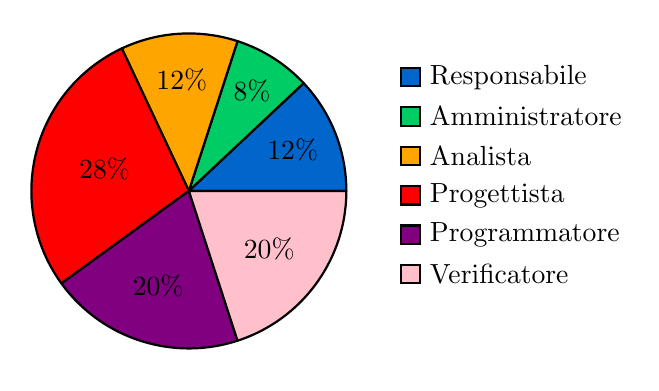
\begin{tikzpicture}
        \pie[
            text=legend,
            color={responsabile, amministratore, analista, progettista, programmatore, verificatore},
            radius=2, % Imposta il raggio per rendere il grafico circolare
            line width=0pt % Rimuovi i contorni
        ]{12/Responsabile, 8/Amministratore, 12/Analista, 28/Progettista, 20/Programmatore, 20/Verificatore}
    \end{tikzpicture}
    \caption{Distribuzione dei costi per ruolo aggiornamento 16/11/2023}
\end{figure}
%------------------------------------------------------------------------

\section{Analisi dei rischi} \label{sec:AnalisiRischi}
\subsection{Descrizione}
Durante lo sviluppo di un progetto è probabile incorrere in problematiche e imprevisti vari. Questi possono provocare effetti indesiderati, quali:

\begin{itemize}
    \item Aumento dei costi previsti per un dato periodo.
    \item Sforamento dei tempi preventivati per la realizzazione dei vari compiti.
    \item Rendimento complessivo condizionato negativamente.
    \item Deterioramento della qualità del prodotto.
\end{itemize}

È necessario quindi attuare un processo utile ad indentificare i rischi ed avere un piano di contingenza per mitigarli o eliminarli.
%------------------------------------------------------------------------

%------------------------------------------------------------------------
\subsection{Processo di mitigazione}
\subsubsection{Identificazione}
Individuare le possibili problematiche che potrebbero verificarsi durante lo sviluppo del progetto. 
Le fonti dalle quali potrebbero derivare i rischi sono: 
\begin{itemize}
    \item Gruppo: collaborazione, comunicazione, competenze tecniche, organizzazione.
    \item Prodotto del capitolato: requisiti, tecnologie, strumenti.
\end{itemize}
%------------------------------------------------------------------------

%------------------------------------------------------------------------
\subsubsection{Processo di analisi}
Per ogni rischio identificato assegnare un indice identificativo e stabilire secondo i seguenti parametri:
\begin{itemize}
    \item Probabilità di occorrenza: quanto è probabile che il rischio si verifichi.
    \item Grado di pericolosità: quali effetti negativi potrebbe causare nello sviluppo del progetto.
\end{itemize}
%------------------------------------------------------------------------

%------------------------------------------------------------------------
\subsubsection{Pianificazione}
Per ogni rischio identificato, definire un piano di contingenza che preveda:
\begin{itemize}
    \item Strategia preventiva: definire le azioni da intraprendere per prevenire l’insorgenza del rischio.
    \item Riduzione dell'impatto: stabilire le misure da adottare per ridurre al minimo l'impatto del rischio, nel caso non si riesca ad evitarlo.
\end{itemize}
%------------------------------------------------------------------------

%------------------------------------------------------------------------
\subsubsection{Processo di controllo e aggiornamento}
Effettuare un monitoraggio periodico delle attività in corso e degli artefatti prodotti, al fine di identificare potenziali nuovi rischi o modificare quelli preesistenti, aggiornando di conseguenza le relative strategie di mitigazione.
%------------------------------------------------------------------------


\begin{comment}
Qui dentro viene mostrato il codice dei rischi che andrà normato nella sezione Gestione dei Rischi nel file Norme di Progetto.
Il rischio ha il seguente codice:   R[Tipo]-[Probabilità][Priorità]-[Indice]

R: rischio
Tipo: natura del rischio (tecnologico (T), organizzativo (O), personale (P), requisiti (R))
Probabilità: probabilità di occorrenza (Alta(1), Media(2), Bassa(3))
Priorità: grado di pericolosità  (Alta(A), Media(M), Bassa(B))
Indice: numero progressivo che identifica il rischio (1, 2, 3, ecc..)

\end{comment}

\subsection{Rischi previsti}
Di seguito sono riportate le tabelle relative ai rischi previsti che potrebbero presentarsi durante lo sviluppo del progetto. \\
La convenzione utilizzata per la codifica dei rischi è la seguente: 
\begin{center}
    \texttt{R[Tipologia]-[Probabilità][Priorità]-[Indice]} : \textit{Nome associato al rischio}
\end{center} 

\begin{flushleft}
    \textbf{Tipologia}: natura del rischio:
    \begin{itemize}
        \item \textbf{T}: Rischi legati all'utilizzo delle tecnologie
        \item \textbf{O}: Rischi legati all'organizzazione del gruppo
        \item \textbf{P}: Rischi legati agli impegni personali dei membri del gruppo
    \end{itemize}
    \textbf{Probabilità}: valore alfabetico che indica la probabilità di occorrenza del rischio:
    \begin{itemize}
        \item \textbf{1}: Alta
        \item \textbf{2}: Media
        \item \textbf{3}: Bassa
    \end{itemize}
    \textbf{Priorità}: valore numerico che indica la pericolosità del rischio:
    \begin{itemize}
        \item \textbf{A}: Alta
        \item \textbf{M}: Media
        \item \textbf{B}: Bassa
    \end{itemize}
    \textbf{Indice}: valore numerico incrementale che determina univocamente il rischio per ogni tipologia di rischio. 
\end{flushleft}


%------------------------------------------------------------------------
\newpage
\subsubsection{Impegni personali e accademici}
\begin{table}[h]
    \centering
    \begin{tabularx}{\textwidth}{l>{\RaggedRight}X>{\RaggedRight}X>{\RaggedRight}X>{\RaggedRight}X}
    \toprule
    \rowcolor{gray!50}
    \textbf{Codice} & \textbf{Descrizione del rischio} & \textbf{Identificazione} & \textbf{Mitigazione} \\
    \midrule
    \addlinespace 
    RO-1A-1 & 
    Rischio di rallentamento del progetto dovuto all'armonizzazione delle attività personali e progettuali, con particolare intensificazione durante la sessione invernale 2023-2024 a causa degli esami. & 
    I membri del gruppo comunicheranno al responsabile i loro impegni durante le riunioni di organizzazione o al momento immediato della conoscenza dell'impedimento.& 
    Il responsabile, considerando gli impegni dei membri del gruppo, avrà la facoltà di riassegnare le varie attività ad altri membri o estendere il tempo previsto per l'esecuzione dell'attività assegnata. \\  
    \bottomrule
    \addlinespace 
    \end{tabularx}
\end{table}

%------------------------------------------------------------------------
\subsubsection{Variazione dei requisiti del progetto}
\begin{table}[h]
    \centering
    \begin{tabularx}{\textwidth}{l>{\RaggedRight}X>{\RaggedRight}X>{\RaggedRight}X>{\RaggedRight}X}
    \toprule
    \rowcolor{gray!50}
    \textbf{Codice} & \textbf{Descrizione del rischio} & \textbf{Identificazione} & \textbf{Mitigazione} \\
    \midrule
    \addlinespace 
    RO-3A-2 & 
    Potrebbero verificarsi modifiche in corso d'opera dei requisiti del progetto, che potrebbero determinare un cambiamento di direzione delle attività. &
    Attraverso le riunioni periodiche con la proponente, vengono comunicate in modo esplicito al gruppo le modifiche di alcuni requisiti.&
    Redigere un'analisi dettagliata dei requisiti all'inizio al fine di identificare e soddisfare completamente le esigenze della proponente. Presentare tali requisiti e attuare tempestivamente eventuali misure correttive necessarie. \\
    \bottomrule
    \addlinespace 
    \end{tabularx}
\end{table}
%------------------------------------------------------------------------
\newpage
\subsubsection{Ritardo nel completamento delle attività rispetto ai tempi previsti}
\begin{table}[h]
    \centering
    \begin{tabularx}{\textwidth}{l>{\RaggedRight}X>{\RaggedRight}X>{\RaggedRight}X>{\RaggedRight}X}
    \toprule
    \rowcolor{gray!50}
    \textbf{Codice} & \textbf{Descrizione del rischio} & \textbf{Identificazione} & \textbf{Mitigazione} \\
    \midrule
    \addlinespace 
    RO-2M-2 & 
    L'inesperienza del gruppo in un progetto software professionale potrebbe portare a superare i tempi preventivati, specialmente a causa della nuova tecnologia e della necessità di migliorare la gestione delle risorse.& 
    I membri del gruppo devono segnalare al responsabile eventuali difficoltà nel rispettare le scadenze previste per le attività. &
    Il responsabile, considerando le motivazioni del ritardo, avrà la facoltà di riassegnare le varie attività ad altri membri o estendere il tempo previsto per l'esecuzione dell'attività assegnata. \\
    \bottomrule
    \addlinespace 
    \end{tabularx}
\end{table}

%------------------------------------------------------------------------

\subsubsection{Apprendimento ed utilizzo delle nuove tecnologie} \label{sec:rischioTec}
\begin{table}[h]
    \centering
    \begin{tabularx}{\textwidth}{l>{\RaggedRight}X>{\RaggedRight}X>{\RaggedRight}X>{\RaggedRight}X}
    \toprule
    \rowcolor{gray!50}
    \textbf{Codice} & \textbf{Descrizione del rischio} & \textbf{Identificazione} & \textbf{Mitigazione} \\
    \midrule
    \addlinespace 
    RT-1A-1 & 
    L’apprendimento e l'implementazione delle tecnologie proposte possono rappresentare un rischio considerevole per lo  sviluppo di un progetto, in quanto esista la possibilità che lo studio accurato di queste tecnologie richieda più tempo del previsto.& 
    I membri del gruppo sono tenuti a notificare tempestivamente al responsabile qualsiasi difficoltà riscontrata durante il processo di studio delle tecnologie proposte. &
    Ogni membro deve studiare le nuove tecnologie, e in caso di difficoltà, organizzare workshop interni e sfruttare le opportunità di formazione dell'azienda proponente. \\
    \bottomrule
    \addlinespace 
    \end{tabularx}
\end{table}

%------------------------------------------------------------------------
\newpage
\subsubsection{Perdita di file}
\begin{table}[h]
    \centering
    \begin{tabularx}{\textwidth}{l>{\RaggedRight}X>{\RaggedRight}X>{\RaggedRight}X>{\RaggedRight}X}
    \toprule
    \rowcolor{gray!50}
    \textbf{Codice} & \textbf{Descrizione del rischio} & \textbf{Identificazione} & \textbf{Mitigazione} \\
    \midrule
    \addlinespace 
    RT-3M-2 & 
    È presente il rischio che alcuni file vengano persi a causa di malfunzionamenti hardware o errori umani. &
    Il danneggiamento o l'eliminazione accidentale di file su cui i membri hano lavorato che compromette il lavoro svolto su quei documenti. &
    Adottare un sistema di versionamento dei file fornisce ai membri del gruppo la capacità di tracciare e recuperare agevolmente versioni precedenti dei documenti, garantendo una robusta protezione contro modifiche indesiderate, danneggiamenti o eliminazioni accidentali.\\
    \bottomrule
    \addlinespace 
    \end{tabularx}
\end{table}

%------------------------------------------------------------------------
\subsubsection{Contrasti interni al gruppo}
\begin{table}[h]
    \centering
    \begin{tabularx}{\textwidth}{l>{\RaggedRight}X>{\RaggedRight}X>{\RaggedRight}X>{\RaggedRight}X}
    \toprule
    \rowcolor{gray!50}
    \textbf{Codice} & \textbf{Descrizione del rischio} & \textbf{Identificazione} & \textbf{Mitigazione} \\
    \midrule
    \addlinespace 
    RP-2B-1 & 
    La comunicazione inefficace tra i membri del gruppo potrebbe causare ritardi significativi nello sviluppo del progetto, specialmente data la natura collaborativa del lavoro di gruppo, che richiede il rispetto di norme concordate collettivamente.& 
    Clima di disaccordo tra i membri del gruppo evidente, con segnali di divergenze di opinioni e contrasti nelle dinamiche di collaborazione. Si manifesta attraverso la mancanza di convergenza di idee, complicando il processo decisionale. &
    Il responsabile è tenuto a mitigare il clima di disaccordo e a perseguire una soluzione che soddisfi la maggioranza dei membri del gruppo. \\
    \bottomrule
    \addlinespace 
    \end{tabularx}
\end{table}

%------------------------------------------------------------------------
\newpage
\subsubsection{Contatti con la proponente}
\begin{table}[h]
    \centering
    \begin{tabularx}{\textwidth}{l>{\RaggedRight}X>{\RaggedRight}X>{\RaggedRight}X>{\RaggedRight}X}
    \toprule
    \rowcolor{gray!50}
    \textbf{Codice} & \textbf{Descrizione del rischio} & \textbf{Identificazione} & \textbf{Mitigazione} \\
    \midrule
    \addlinespace 
    RP-3M-2 & 
    La comunicazione con l'azienda proponente potrebbe non essere più efficace e potrebbe non essere sempre possibile, il che potrebbe portare alla comparsa di dubbi e richieste. & 
    Le risposte assenti o incomplete non contribuiscono alla risoluzione dei dubbi o delle domande proposte. Frequenza degli incontri che diminuisce.&
    Il responsabile è tenuto a comunicare la situazione alla parte proponente, cercando di trovare una soluzione. Se non si riesce a risolvere il problema con la parte proponente, si richiederà l’intervento del committente. \\
    \bottomrule
    \addlinespace 
    \end{tabularx}
\end{table}
%------------------------------------------------------------------------

\section{Pianificazione, preventivo e consuntivo}
\subsection{Pianificazione}
In conformità con la filosofia di sviluppo moderna e dinamica, abbiamo scelto di adottare il modello agile, con un focus specifico sul framework Scrum.
Lo Scrum, con le sue pratiche iterative e collaborative, offre una risposta efficace alle sfide e alle mutevoli esigenze del mondo contemporaneo dello sviluppo software.\\
Attraverso l'implementazione di Scrum, il nostro team mira a ottenere numerosi benefici positivi che influenzeranno in modo significativo il successo del progetto.
\\
\\
\textbf{Vantaggi del Modello Agile e Scrum}
\\L'adozione del modello Agile, e in particolare di Scrum, introduce una serie di lati positivi che contribuiranno al raggiungimento dei nostri obiettivi di progetto.
Alcuni dei principali vantaggi che ci aspettiamo di acquisire includono:

\begin{itemize}
    \item \textbf{Flessibilità e Adattabilità:} Lo Scrum consente una rapida risposta ai cambiamenti nei requisiti del cliente, garantendo una maggiore flessibilità durante tutto il ciclo di sviluppo;
    \item \textbf{Collaborazione e Comunicazione:} La struttura collaborativa di Scrum promuove una comunicazione aperta e continua tra i membri del team e le parti interessate, migliorando la comprensione reciproca e la condivisione di conoscenze;
          \begin{itemize}
              \item In particolare con l'azienda proponente sono fissati SAL (Stato avanzamento lavori) ogni due settimane.
          \end{itemize}
    \item \textbf{Consegna Incrementale:} Attraverso la pratica di rilasci incrementali, Scrum consente la distribuzione graduale delle funzionalità, fornendo valore al cliente fin dalle prime fasi del progetto;
    \item \textbf{Miglioramento Continuo:} Le retrospettive regolari incoraggiano il miglioramento continuo del processo, permettendo al team di identificare e risolvere eventuali problematiche in modo tempestivo.
\end{itemize}

La scelta di adottare il modello Agile con Scrum riflette la nostra dedizione a fornire un prodotto di qualità, rispondendo in modo efficiente ai cambiamenti e alle esigenze del cliente.

\subsection{Preventivo}
Un preventivo è un documento ufficiale che fornisce una stima dettagliata delle risorse necessarie per condurre le attività pianificate. Questo documento include una previsione riguardante il consumo di risorse, tenendo debitamente conto dei costi economici e temporali sostenuti dal gruppo in ciascun periodo di attività.
\subsection{Consuntivo}
Un consuntivo è un documento ufficiale che riporta in dettaglio le attività effettivamente eseguite e i costi (economici e temporali) effettivamente sostenuti durante un periodo di attività specifico.

\subsection{Gestione e monitoraggio dell'avanzamento del Progetto}
In collaborazione con la proponente, si è concordato di organizzare l'avanzamento del progetto in periodi di due settimane, seguendo un approccio simile agli sprint di Scrum. Durante ciascun periodo, verranno selezionate, in collaborazione con l'azienda e i membri del team, le attività da svolgere.
La scelta delle task si baserà sulla loro importanza strategica e sulla fattibilità di completarle entro la durata del periodo. Nel caso in cui alcune attività non vengano portate a termine entro il periodo, verranno riportate nel consuntivo di periodo e proseguiranno nel periodo successivo.
Ogni periodo sarà documentato attraverso una tabella esaustiva in cui saranno identificate le task relative a ciascun ruolo. Per ogni attività, verrà indicato lo stato di completamento, i tempi previsti ed effettivi, e i costi associati.
\\Le attività assegnate al ruolo "Team" non vengono considerate nel computo dei costi, in quanto sono associate a iniziative di carattere interno e possono essere eseguite da ruoli vari.
\\ Le ore impiegate per tali attività sono regolarmente registrate nella sezione "Preventivo orario per membro" presente in ciascun periodo.
\\Al termine di ciascun periodo, sarà calcolato il costo totale fino a quel momento del progetto, fornendo una chiara visione del progresso complessivo.
\\Inoltre ogni periodo conterrà una discussione sui rischi occorsi e sull'esito della loro mitigazione seguendo quanto definito in (\ref{sec:AnalisiRischi})\\
I dati riportati in ogni periodo sono il resconto di quanto inserito in autonomia dai membri nel foglio google condiviso disponibile
\href{https://docs.google.com/spreadsheets/d/1gbGCTKO6tLKN7lI9kTZHLpoItniJIi9X/edit?usp=sharing&ouid=104272518979154193028&rtpof=true&sd=true}{qui}.


\subsection{Requirements and Technology Baseline}
\subsubsection{Primo periodo  06/11/2023 - 24/11/2023}
Nel corso del primo periodo, il nostro team ha dedicato risorse significative all'elaborazione e alla standardizzazione dei processi, formalizzando tali linee guida nel documento "Norme di Progetto". In quest'ultimo, sono state dettagliatamente redatte le sezioni specificate nella tabella sottostante.
Durante il primo incontro con l'azienda, abbiamo definito obiettivi chiave da conseguire entro il prossimo SAL fissato per il 24 novembre 2023, coincidente con l'avvio del prossimo periodo. Questo approccio ricalca la struttura dello sprint backlog di Scrum.
Tra i molteplici obiettivi delineati, si evidenziano la realizzazione di almeno un simulatore di un sensore in linguaggio Python, il quale interagisca con un server Kafka mediante Docker. Opzionalmente, si è prevista l'integrazione con il database ClickHouse per immagazzinare i dati dei simulatori. In parallelo, ci si è dedicati alla creazione di user story e casi d'uso correlati al capitolato.
È soddisfacente constatare che tutte le richieste avanzate dalla proponente sono state risolte entro i tempi concordati, includendo le richieste opzionali.
Parallelamente, durante questa fase, gli amministratori hanno investito risorse per automatizzare il processo di compilazione dei sorgenti LaTeX, una volta caricati nella repository condivisa. Inoltre, è stata implementata una procedura automatica di rinomina dei file PDF generati, inclusiva dell'indicazione della versione.

\paragraph{Rischi occorsi, impatto, mitigazione}

Nel corso del primo periodo, si sono presentate le seguenti problematiche:
\begin{itemize}
    \item \textbf{Inesperienza nell'uso dell'ambiente Docker - \ref{sec:rischioTec}}
          \begin{itemize}
              \item \textbf{Esito mitigazione:}  L'autoapprendimento e la conoscenze dei singoli non si sono dimostrate adeguate per acquisire una conoscenza approfondita dell'ambiente Docker nel breve periodo iniziale,
                    portando all'utilizzo del sistema senza una comprensione approfondita di ciascuna delle sue componenti e configurazioni. Di conseguenza,
                    è stata formulata una richiesta al proponente per la realizzazione di un corso di formazione specifico su Docker seguendo le norme di mitigazione definite in \ref{sec:rischioTec}.
              \item \textbf{Impatto:} Nessuna conseguenza significativa è stata riscontrata, poiché le avvertenze segnalate dalla proponente riguardavano criticità di lieve entità relative alle best practices di Docker. Le misure di mitigazione necessarie sono state tempestivamente implementate, e un incontro formativo è stato programmato per approfondire ulteriormente la questione.
                    Inoltre, al fine di conformarsi alle best practices dell'ambiente, è stata presa la decisione di regolamentare, nel documento "Norme di Progetto", lo sviluppo degli ambienti Docker.
          \end{itemize}
\end{itemize}
\paragraph{Pianificazione attività divise per ruoli con consuntivo e preventivo orario e dei costi}\hspace{1pt}

\begin{figure}[H]
    \centering
    \includegraphics[height=1.1\textwidth]{../Images/periodo1.jpg}
    \caption{Primo periodo}
    \label{fig:1periodo}
\end{figure}

Al termine del primo periodo, l'ammontare parziale totale del costo del progetto è \textbf{ 1093\euro\ } e sono state completate il \textbf{100\%} delle attività attese.

\begin{figure}[h]
    \centering
    \begin{minipage}[b]{0.45\textwidth}
        \centering
        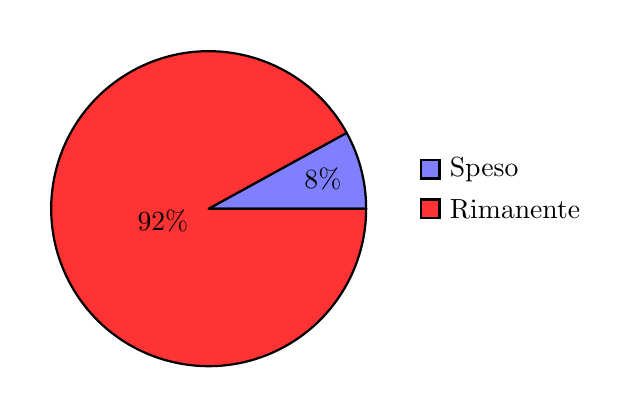
\begin{tikzpicture}
            \pie[
                text=legend,
                color={blue!50, red!80}, % Sostituisci con i colori desiderati
                radius=2, % Imposta il raggio per rendere il grafico circolare
                line width=0pt % Rimuovi i contorni
            ]{8/Speso, 92/Rimanente}
        \end{tikzpicture}
        \caption{Grafico a torta del budget speso e rimanente preventivato nel primo periodo}
        \label{fig:GraficoTorta}
    \end{minipage}

    \vspace{1cm} % Aggiungi spazio verticale tra le due figure

    \begin{minipage}[b]{0.70\textwidth}
        \centering
        \includegraphics[width=0.7\textwidth]{../Images/avanzamento1Periodo.png}
        \caption{Avanzamento dei lavori RTB - primo periodo}
        \label{fig:AvRtb1}
    \end{minipage}
\end{figure}

\paragraph{Preventivo e consuntivo orario per membro}
Nel corso del primo periodo, sono state impiegate ore per l'esecuzione di attività interne, come dettagliato nella tabella precedente. Tali ore non sono state incluse nei costi e per svolgerle sono intervenuti i ruoli di responsabile e amministratore.
Per le attività registrate nei costi, sono stati assegnati i seguenti ruoli:

\begin{itemize}
    \item \textbf{Responsabile (Re):}
          \begin{itemize}
              \item F. Pozza.
          \end{itemize}
    \item \textbf{Amministratore (Am):}
          \begin{itemize}
              \item L. Skenderi.
          \end{itemize}
    \item \textbf{Analisti (An):}
          \begin{itemize}
              \item A. Barutta;
              \item R. Smanio.
          \end{itemize}
    \item \textbf{Verificatore (Ve):}
          \begin{itemize}
              \item E. Hysa.
          \end{itemize}
    \item \textbf{Programmatori (Pr):}
          \begin{itemize}
              \item N. Preto;
              \item D. Diotto.
          \end{itemize}
    \item \textbf{Progettista (Pt):}
          \begin{itemize}
              \item Nessuno.
          \end{itemize}
\end{itemize}

\paragraph{Preventivo orario} \hspace{1pt}

\begin{figure}[h]
    \centering
    \includegraphics[width=0.9\textwidth]{../Images/preventivoOrario1Periodo.png}
    \caption{Preventivo orario per membro - primo periodo}
    \label{fig:Pv1}
\end{figure}

\begin{figure}[H]
    \centering
    \includegraphics[width=0.7\textwidth]{../Images/preventivoDivisioneRuoli1Periodo.png}
    \caption{Istogramma preventivo della ripartizione oraria dei ruoli - primo periodo}
    \label{fig:PvD1}
\end{figure}

\paragraph{Consuntivo orario } \hspace{1pt}

\begin{figure}[h]
    \centering
    \includegraphics[width=0.9\textwidth]{../Images/consuntivoOrario1Periodo.png}
    \caption{Consuntivo orario per membro - primo periodo}
    \label{fig:Cv1}
\end{figure}

\begin{figure}[H]
    \centering
    \includegraphics[width=0.7\textwidth]{../Images/consuntivoDivisioneRuoli1Periodo.png}
    \caption{Istogramma consuntivo della ripartizione oraria dei ruoli - primo periodo}
    \label{fig:PvD1}
\end{figure}

\end{document}
